\documentclass{article}
\usepackage{graphicx}
\usepackage{amsmath, amsthm, amssymb, amsfonts, amsbsy}

\begin{document}
\section{Methods}
For millennia, humans (and other animals) have tried to understand the rules that govern the phenomena surrounding them based on observations. This knowledge allowed them to expand the reach of their predictions and develop inventions to improve their way of living, as well as the empirical laws that support all the fields of fundamental science, and consequently applied science. In the last 5 decades, with the advent of several kinds of sensors, fast electronics and large storage capacity, quantitative observations have become more and more numerous at a great level of detail (the "deluge of data") [ref] and it appears that this way of learning is becoming more and more necessary in the present than ever before.

Datasets became very large in the number of elements as well as very high in its dimensionality (the "Deluge of Data"), in a such way that they are no longer amenable for a human operator to analyze them. To be able to deal with this problem, researchers and engineers started using computers in particular methods of Machine Learning. Machine Learning is a subfield of computer science that studies and develops algorithms meant to find new structures or rules a given experiment or phenomenon is based on. Arthur Samuel defined machine learning as a "Field of study that gives computers the ability to learn without being explicitly programmed" (reference Phil Simon (March 18, 2013). Too Big to Ignore: The Business Case for Big Data. Wiley. p.89. ISBN 978-1-118-63817-0.)

However, conventional machine learning techniques often require careful and domain-specific design in order to achieve good results. For example, it usually takes a considerable amount of expertise and experience with a phenomenon of interest in order to determine an algorithm and/or model that would be a good approximation of what was actually happening in the experiment under study

In the field of statistical machine learning, a dataset consists of m points (examples), each one with a set of n features defining a n-dimensional space (input space). Depending on the specific kind of model we would like to extract from the data, there are a number of different approaches for machine learning.

The most commonly used form of machine learning uses labeled datasets. This is called supervised learning.

\subsection{Supervised Learning}
\label{subsec:supervised-learning}

In supervised learning, each input example has an extra feature that represents the “true” value, the "right answer" we would like to obtain from the machine for this instance. If the dataset has such features, it is said to be labeled, otherwise, it is unlabeled.

Supervised learning algorithms are usually iterative methods. They are usually presented with a large number of labeled examples beforehand, which they then use to modify the evaluation model in order to output the best possible answer [what is a model? a definição devia aparecer antes]. These modifications follow a set of operations (the training or learning algorithm), that depends on some measure of dissimilarity between the outputs of the model in its current configuration (the model predictions) and the corresponding labels. This function is usually called a loss function and is most often thought of as a distance. Examples of loss functions are the Mean-Squared Error of Cross Entropy [others?]. At each iteration, the training algorithm will calculate the necessary adjustments in order to make the loss function smaller. After a certain number of iterations, the algorithm will, possibly, converge on a solution that is a good enough approximation of the results a human supervisor would produce when analyzing the same dataset.

In machine learning, we must choose a model (or framework) to work with. In the case of linear regression, the output of the algorithm is a linear function of the form $y = mX + b$, where m and b are the adjustable parameters. This choice strongly conditions the power of the algorithm. If, for instance, y depends on $X$ quadratically, linear regression may not yield the best results; however, depending on the situation it may provide a good enough approximation.
Another choice the user must define a priori is the training algorithm. A simple example of such an algorithms is gradient descent. 

In supervised learning we are not only interested in producing a model for the data we do have but more generally in predicting the outcome of the experiment in untested situations that we have yet to observe.

More formally, the computer receives a number, m, of examples of input as a (n-dimensional) feature vectors $\vec{x_i}, i = 1,2, \ldots ,m$ and corresponding (p-dimensional) target (“true”) value $\vec{ y_i}, i=1,2, \ldots ,m$ and tries to find the element in the family of functions (hypothesis class) $h_{\theta}$ parameterized by $\theta$ such that $\vec{ y_i}  \approx h_\theta \left(\vec {x_i} \right)$ for each example. 

\subsubsection{Linear Regression}
\label{subsubsec:linear-regression}
In the context of linear regression, we restrict ourselves to a family of function such that:
\begin{equation}
h_{\vec{\theta},b} ( \vec{x} ) = \sum_{j = 1}^{m} \theta_j x_j + b = \theta \cdot \vec{x} + b
\end{equation}
where $\theta$ and $b$ are the parameters to be learnt.

A common choice for the loss function is the Mean Squared Error (MSE), defined as:

\begin{equation}
J \left( \theta , b\right) = \frac{1}{2} \sum_{j=1}^m \left[ h_{\theta,b} \left( \vec{x}^{(j)} \right) -  y^{(j)} \right]^2 =  \frac{1}{2} \sum_{j=1}^m \left( \theta \cdot \vec{x}^{(j)} + b - y ^{(j)} \right) ^2
\label{eq:MSE-definition}
\end{equation}

Most training algorithms require the knowledge of the gradient of the loss function with respect to the model's parameters to determine the update rule. In this situation, the gradient would be:

\begin{eqnarray}
\frac{ \partial J}{\partial \theta_i } &=& \sum _{j= 1}^m x_i^{(j)} (  h_{\theta, b} ( x^{(j)}) - y^{(j)} ) \\
\frac{ \partial J}{\partial b } &=&  \sum _{j= 1}^m (  h_{\vec{\theta}, b} ( x^{(j)}) - y^{(j)} )
\label{eq:MSE-gradient}
\end{eqnarray}

And the parameters would be updated as:
\begin{eqnarray}
\theta_i^{n+1} &=& \theta_i^{n} - \eta \left[\nabla_{\theta} J(\theta^n,b^n )\right]_i \\
b^{n+1} &=& b^n - \eta \frac{\partial J}{\partial b} \left(\theta^n,b^n \right)
\label{eq:GD-update-rule}
\end{eqnarray}
where $\eta$ is the learning rate defined by the user.


\subsubsection{Logistic Regression}
\label{subsubsec:Logistic-Regression}
Machine learning is also often used to perform a classification task where we are trying to assign a class (discrete value) to some input vector. For instance, we could apply linear regression and set a  threshold value to define the boundary between two class. However this method is very sensitive to extreme values of the input. In the case of binary classification $y^{(i)}$ can only be either 1 or 0. In this situation Logistic Regression is usually a better choice. With logistic regression we try to find the predictor choosing a different hypothesis class: 
\begin{equation}
h_{ \theta, b } (x) = \sigma ( \theta \cdot x + b) = \frac{1}{ 1 + exp(-\theta \cdot x - b) }
\label{def:logistic-regression}
\end{equation}
Note that this function (called the sigmoid function or logistic function) is a continuous for all values of $x$. It is always positive, monotonically increasing from zero to one. This leads to the interpretation of the output of the logistic regression as the probability of the class labeled as “1” happening given the input vector x: 
\begin{eqnarray}
P( Y=1 \mid  X = x ) &=& \frac{1}{ 1 + \exp(-\theta \cdot x - b)} \leqslant 1 \\
P( Y=0 \mid  X = x ) &=& 1 - P( Y=1 \mid  X = x )
\end{eqnarray}

The cost function in this case is usually defined as:
\begin{equation}
J(\theta,b) = - \sum _{j= 1}^m ( y^{(j)} \log(h_{\theta,b}(x^{(j)})) + (1-y^{(j)}) \log(1- h_{\theta,b}(x^{(j)})) )
\end{equation}

Since in this setup $y^{(j)}$ can only be either 1 or 0, only one of the terms inside the summation is non-zero.

The gradient of this loss function is:
\begin{equation}
\nabla _{\theta,b} J(\theta,b) = \sum _{j= 1}^m x^{(j)} ( h_{\theta,b}(x^{(j)}) - y^{(j)} )
\end{equation}

In classification tasks it is common to have more than two classes that we are interested in. In this case, we can generalize logistic regression to many-classes using Softmax Regression, where the probabilistic interpretation is applied

In classification task, we are looking for the boundary between classes in the feature space. The techniques I mentioned above can only resolve problems in which the classes are linearly separable (where the boundary is an hyper-plane in the feature space). But this is not always the case. Sometimes the region corresponding to a particular class may even be disjoint. In such case linear classifiers are not powerful enough to solve the problem. (As an example consider the Exclusive OR function where the inputs are two binary valued variables. There is not straight line in the input space that separates the class “0” and the class “1”.)

\subsection{Artificial Neural Networks}
\label{subsec:ANN}

A much more powerful concept is that of Artificial Neural Networks. 
An artificial neuron (hereafter neuron unless stated otherwise) is a computational unit that takes as input the vector $x$ and outputs
\begin{equation}
h_{w,b} (x) = f\left( w \cdot x + b \right) = f \left( \sum_{i=1}^n w_i x_i + b  \right)
\end{equation}

where $f\colon \textbf{R} \rightarrow \textbf{R}$ is called the activation function. The vector $\textbf{w}$ and the value of b (called the bias or intercept term), as before, can be tuned according to some algorithm to perform a designated task as good as possible. 

If the activation function is the sigmoid function we recover the logistic regression.

Another example of activation function is the hyperbolic tangent, which increases from -1 to 1. 
Lately, researchers and engineers have started using the rectified linear function (RELU) particularly in the context of deep neural network (which I'll talker later in this document). This function is defined as
\begin{equation}
RELU(z)= \max(z,0) = 
\begin{cases}
    z,& \text{if } z\geq 0\\
    0,              & \text{if } z < 0
\end{cases}
\end{equation}

This activation function is significantly different from the ones referred before because it is not bounded as $z$ increases. Moreover, it is not differentiable when $z=0$ although this doesn't become a problem in practice because it is differentiable at any point arbitrarily close to 0.

A Artificial Neural Network (ANN) is put together by hooking together many of these simple neurons by means of function composition where the output of one neuron is the input of another.


\begin{figure}[!h]
	\centering
	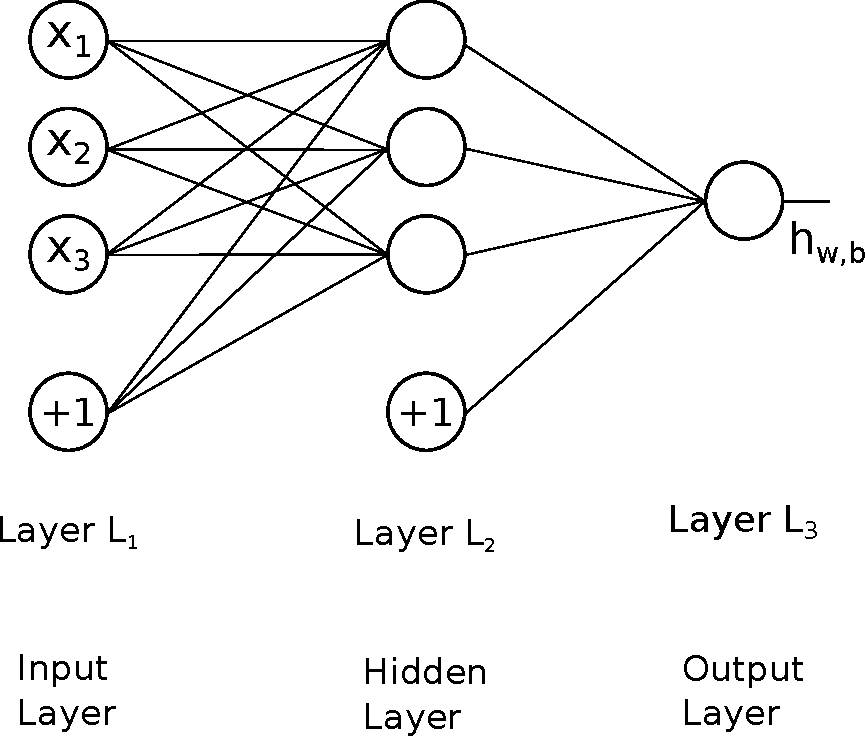
\includegraphics[width=\linewidth]{firstANN.pdf}
	\caption{Graphical visualization of an illustrative example of an artificial neural network. This ANN is composed by three layers with three neurons on the first two and one neuron on the output layer. The connections between all the neurons are also represented, in addition to the connection to the bias term represented by the extra nodes on the bottom with the label "+1".
}
\label{fig:first-ANN}
\end{figure}
In the Fig. \ref{fig:first-ANN} is a graphical representation of what was just mentioned. On the left, we have the input layer (layer $L_1$) where the input vector $(x_1,x_2,x_3)$ is fed. In the middle there are three neurons. These are called hidden neurons and they compose one hidden layer ($L_2$). Finally, there is the output layer with only one neuron. There are also two nodes on the bottom that represent the bias term.

In this example, there are connections between all neurons of one layer to the neurons in the next layer. This ANN is said to be fully connected (or densely connected). For each connection there is an associated parameter (weight) and also a bias parameter. The input of each neurons in the hidden layer is a linear combination of the output of the neurons in the previous layer weighted by the parameters of the corresponding connections and summed with the bias term. In this case, the weights for the connections coming in to the first neuron in the layer L2 are $w_{1,1}^{(1)},w_{1,2}^{(1)},w_{1,3}^{(1)}, b_1^{( 1 )}$ and its input is:
\begin{equation}
z_1^{(2)} = \sum_{i=1}^3 w_{1,i}^{(1)} a_i^{(1)} + b_1^{(1)}
\end{equation}
This input is then fed into the activation function which reveals the outputs of this neuron as 
\begin{equation}
a_1^{( 2 )} = f\left( z_1^{(2)} \right)
\end{equation}

We denoted the number of layer as $n_l$ and the number of neurons in the layer $L_l$ as $S_l$. In the example above $n_l=3$, $S_1 = S_2 = 3$ and $S_3 = 1$

In general, when the network is densely connected, the input of the neuron i in the layer j is:
\begin{equation}
z_i^{(j)} = \sum_{k=1}^{S_{l-1}} w_{i,k}^{(j)} a_k^{(j-1)} + b_i^{(j-1)}  
\end{equation}
And its output is:
\begin{equation}
a_i^{(j)} = f(z_i^{(j)})
\end{equation}
It is also convenient to introduce a matrix notation such that:
\begin{equation}
\textbf{z}^{(j)} = \textbf{W}^{(j)} \textbf{a}^{(j-1)} + \textbf{b}^{(j-1)}
\end{equation}
where the vector $\textbf{z}^{(j)}$, $\textbf{a}^{(j)}$ and $\textbf{b}^{(j)}$ represent the input, output and bias parameter of all neurons in Layer $L_j$

The output of the output layer is denoted $\textbf{h}_{\textbf{W},\textbf{b}}\left( \cdot \right) = \textbf{a}^{(L)}\left( \cdot \right)$


Using Artificial Neural Networks, we now have a much more powerful and flexible framework to create models that can be trained to compute much more complex functions than the ones computable with traditional machine learning algorithms.

However, there's still the need to define the training algorithm. In order to use the gradient descent algorithm, it is necessary to compute the gradients of the loss function with respect to all the adjustable parameter of ANN. These gradients are usually computed using the back-propagation algorithm. In this method, the label is subtracted from the output value as an estimate of the gradient on the output layer. This value is then propagated backwards layer by layer by applying the chain rule for derivatives, which will depend on the chosen activation functions. With the gradients estimated, the parameters are update in the way defined earlier in equation \ref{eq:GD-update-rule}

The key aspect of learning with ANN is that, due to its generalization power, the form of the final output function is not directly designed by a human: they are learned from the data.

But this framework leads to questions of how exactly to define the model. In other words, how to define the architecture of the ANN, i.e., how many neurons should there be in the ANN and how should they be connected? There are two basic topologies: shallow networks and deep networks. In shallow networks, there is at most one hidden layer, whereas a network is said to be deep if it has two or more hidden layers. This distinction has become very important over the last three decades. On the one hand, it has been shown that a shallow ANN with only one arbitrarily large hidden layer could approximate a function to any level of precision (REFERENCE Horniket al.,1989). Nonetheless, this level of precision would only increase with exponentially increasing number of neurons, becoming computationally very demanding.

On the other hand, deep neural networks are conceptually more interesting because each layer can be thought of as a representation of the input in a higher and higher level of abstraction, similar to how the visual processing hierarchy in cortex is thought to operate to construct human visual perception. However, using back-propagation and gradient descent with the usual sigmoid or tanh function can very quickly run into the problem of “vanishing gradients”, when the activation function saturates and the training will not proceed any further. Moreover, even in the cases where training is possible, deep networks were originally found to perform worse than shallow networks.

However, in the past decade there have been several theoretical and technological advances that brought deep neural network back to life.

\subsection{Deep Learning}
\label{subsec:Deep-Learning}
Representation learning is a family of methods that allows machines to find new ways of representing the raw data it was fed with. Deep Learning tries to accomplish this in a "layer by layer" manner. In a deep neural network, each layer holds a new representation of the input data, by transforming the output of the previous layer into a new representation, a more abstract way of perceiving the input data. Composing many of these layer, it should be possible to compute very complex function. For the case of classification task, higher layers of representation may amplify aspects of the input that are important for the discrimination and suppress irrelevant features.

In this section, the techniques used in this project will presented such as training (or optimization), loss function, initialization methods and regularization

\subsubsection{Stochastic Gradient Descent}
\label{subsubsec:SGD}
Stochastic Gradient Descent (SGD) is a stochastic approximation of the gradient descent algorithm described in the previous section. In SGD, only utilizes a subset (called a batch) of the provided examples to compute the gradient. This "noisy" approximation of the gradient is then used to update the parameters of model. It should be noted that all the examples in the dataset are utilized: the entire dataset is split in batches and for each batch there is one update in the parameters. One pass through the entire dataset is called an epoch. This means that there will be more (but faster) iteration than in the standard gradient descent. Surprisingly, this simpler method is known to yield good results much faster than more sophisticated algorithms.

Stochastic learning is often much faster than classic learning particularly when using large redundant datasets: if, for instance, the dataset is composed of the ten repetitions of a smaller set of examples, then estimating the gradient using the whole dataset would have the same result as using one tenth of the dataset. Of course in practice two examples are rarely the same. However many example may be acquisition of the same pattern and therefore will contain approximately the same amount of information.

Networks learn the fastest from examples that are most distant from what the network predicted. Therefore it would preferable to choose such examples in each iteration. Of course, there is no simple way to know which are the "good" examples to train the network with in each iteration. There is a relatively simple way of applying this idea. Assuming successive examples do not differ much, shuffling the dataset before splitting would make the batches "richer" in terms of the information they contain.

Another interesting characteristic of stochastic learning is that it is less prone to get the network stuck in local minima of the loss function. The noise introduced in the gradient estimation generates updates on the parameters that allow easier "jumps" of the parameters from one local minima to another, possibly deeper than the previous. On the other hand, this noise also prevents the full convergence to the minimum: the parameter will always have stochastic fluctuation. This can be address by  adaptively changing the size of the batch or the learning rate.

\subsubsection{AdaGrad}
\label{subsubsec:Adagrad}
One solution for the problem just mentioned is AdaGrad (Adaptive Gradient optimization), proposed in 2011 by Duchi et al. REFERENCE. In this algorithm, the learning rate is adapted in each iteration according to the geometry of the loss function in the vicinity of the current values of the parameters. For each element in the parameter matrix, the user-defined learning rate $\eta$ is weighted by factor that makes it larger or smaller according to a (fast) approximation of the Hessian Matrix. In other words, the update for each parameter is more coarse when far from a local minimum and finer when close to a local minimum.

It should be noted that this algorithm was proposed for convex optimization problems. However, even in non-convex situations AdaGrad usually performs better that standard SGD. (REFERENCE  Gupta, Maya R.; Bengio, Samy; Weston, Jason (2014). "Training highly multiclass classifiers" (PDF). JMLR 15 (1): 1461–1492.)

\subsubsection{Parameter Initialization}

The starting values of the weights can have a significant effect on the training process. For instance, in an ANN with the hyperbolic tangent as activation function, if all parameters were initialized with the same value all neurons would output the same value and get the same updates during training. This would render the network useless. For this reason it is necessary to break these symmetries from the onset.

To get the most out a certain ANN, the initial parameters should be as  uncorrelated as possible. However, if the weights are initialized with very high values, a sigmoid or tanh activation function would start saturated, gradients would vanish and the training wouldn't be possible.
To solve this problem, the initial parameters are usually  sampled from a uniform distribution $U([-a,a])$, where a is some small value. There are several proposals for determining the value of a depending on the particular model chosen by the user: He Uniform, Xavier Uniform(also known as Glorot Uniform) or LeCun Uniform. REFERENCES

For example, LeCun Uniform was defined with sigmoid activation functions in mind. With this initialization method, starting values for the weights are drawn from a uniform distribution with zero mean and standard deviation such that the input of each neuron has a standard deviation close to 1.

\subsubsection{Loss Function}
\label{subsubsec:loss-function}
MSE

cross entropy

\subsubsection{Regularization}

L1 and L2 regularization

Dropout
\end{document}
